\blue{
\section{PhaseFormer-LA}
\label{sec:extension}

\sysLA keeps the conference architecture of Section~\ref{sec:method} unchanged: phase tokenization, embedding, cross-phase routing and the shared predictor are exactly those of \sysname. It adds two components, each derived from one result of Section~\ref{sec:theory}: a level branch on cycle means with its gated fusion (Sections~\ref{sec:ext_branch} and~\ref{sec:ext_fusion}), and a centered amplitude modulation (Section~\ref{sec:ext_modulation}). Figure~\ref{fig:la_overview} shows where they attach.

\begin{figure*}[t]
\centering
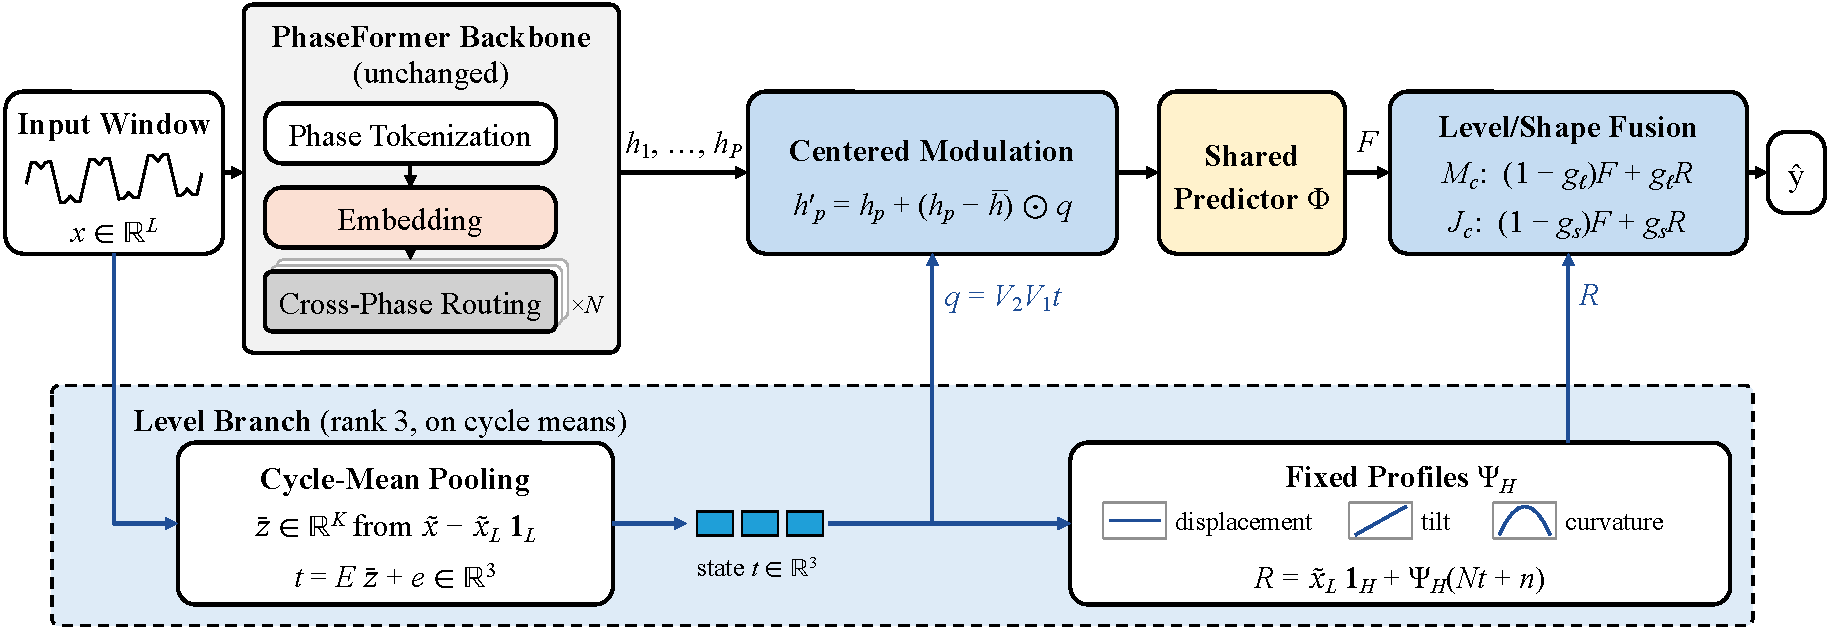
\includegraphics[width=\textwidth]{figures/la_overview.pdf}
\caption{\sysLA. The \sysname backbone and the shared predictor are unchanged and keep their colors of Fig.~\ref{fig:overview}; the new components are blue. A rank-3 level branch reads the anchored cycle means and writes onto three fixed horizon profiles; its state $t$ drives a centered modulation of the final phase latents; the two forecasts are fused with separate level and shape gates.}
\label{fig:la_overview}
\end{figure*}

\subsection{Level branch on cycle means}
\label{sec:ext_branch}

Let $\tilde x_L$ be the last value of the normalized window. The branch pools the anchored window $\tilde x-\tilde x_L\one_L$ to its $K$ cycle means $\bar z\in\mathbb R^K$ and maps them to a rank-3 state,
\begin{equation}
t=E\bar z+e\in\mathbb R^3,\qquad
R=\tilde x_L\one_H+\Psi_H\,(Nt+n),
\label{eq:branch}
\end{equation}
where $\Psi_H\in\mathbb R^{H\times3}$ holds the displacement, tilt and curvature profiles, the discrete orthogonal polynomials of degree $0,1,2$ on the forecast grid, normalized to unit root mean square, so that its first column is $\one_H$ and the other two are horizon-centered. $\Psi_H$ is fixed; only $E\in\mathbb R^{3\times K}$, $e$, $N\in\mathbb R^{3\times3}$ and $n$ are learned. The design follows Theorem~\ref{thm:complement} term by term: the input contains the Bayes level functional, which is a function of the cycle means; the output spans the displacement profile and two smooth profiles; the rank is the number of profiles; and the anchor gives the branch an exactly shift-equivariant level channel that, unlike the phase path's, is not bounded by an envelope. $N$ and $n$ are initialized to zero, so the branch initially forecasts the last value. The branch has $3K+3+9+3=105$ parameters at $K=30$, \emph{independently of the horizon}.

\subsection{Level and shape fusion}
\label{sec:ext_fusion}

Let $F$ be the phase forecast and $R$ the branch forecast, both in normalized units. For every future cycle, the level of the fused forecast and its within-cycle shape are mixed with separate gates,
\begin{equation}
\begin{gathered}
M_c\hat{\tilde y}=(1-g_\ell)M_cF+g_\ell M_cR,\\
J_c\hat{\tilde y}=(1-g_s)J_cF+g_sJ_cR,
\end{gathered}
\label{eq:fusion}
\end{equation}
with $g_\ell=\operatorname{sigmoid}(\omega)$ and $g_s=\operatorname{sigmoid}(\omega+\delta)$. Both gates start at $0.2$ ($\delta=0$). Separate gates let the level be handed to the branch, as Theorem~\ref{thm:complement}(c) prescribes, without forcing the branch's smooth profiles into the phase shape. The gates are static: they depend on neither the input nor the time step. They are learned either per channel ($2C$ parameters) or shared across channels (two parameters); Section~\ref{sec:ext_setup} gives the rule that selects between the two for each dataset.

\subsection{Centered amplitude modulation}
\label{sec:ext_modulation}

Let $h_1,\dots,h_P\in\mathbb R^d$ be the phase latents after the last routing layer. Before the shared predictor, \sysLA modulates them as in \equref{eq:modulation} with a vector driven by the branch state,
\begin{equation}
h'_p=h_p+(h_p-\bar h)\odot q,\qquad q=V_2V_1\,t,
\label{eq:la_modulation}
\end{equation}
with $V_1\in\mathbb R^{k\times3}$, $V_2\in\mathbb R^{d\times k}$, $k=\min(w,3,d)$, no biases, and $V_2$ initialized to zero; the width $w$ is $2$ by default, and the grid search of Section~\ref{sec:ext_setup} also tries $w=4$, which the branch rank caps at $k=3$. The modulation is the complement of Theorem~\ref{thm:amplitude}: centering over the phases is what makes it invisible to every future cycle mean (part~c), and the level-driven factor $q$ scales the shape budget of the phase path (part~d). The branch state $t$ is the natural driver because Theorem~\ref{thm:complement} makes it a linear read of the level forecast. A modulation of width $k=1$ already contains the construction of Theorem~\ref{thm:amplitude}(d); $k=2$ also allows the tilt state to modulate the shape. The modulation has $k(3+d)$ parameters.

\subsection{Properties and cost}
\label{sec:ext_properties}

\fakeparagraph{Exact nesting}
With $V_2=0$ the modulation is the identity, so \sysLA reduces exactly to \sysL; with $g_\ell=g_s=0$ it reduces exactly to \sysname. Because $V_2$ is initialized to zero, \sysLA and \sysL have identical forecasts at initialization when they are built from the same random state, which our experiments use to pair them.

\fakeparagraph{Preserved guarantees}
Theorem~\ref{thm:amplitude}(c) applies to \equref{eq:la_modulation} for every value of $V_1$, $V_2$ and $t$, so the level path of \sysLA is exactly that of \sysL. Theorems~\ref{thm:level_envelope}(b,c) and~\ref{thm:complement} hold for its phase path. The fusion~\equref{eq:fusion} needs whole forecast cycles, which all benchmark horizons provide.

\fakeparagraph{Parameters and complexity}
The branch adds 105 parameters and the modulation $k(3+d)$, so together they add between 119 and 367 parameters across all 28 settings, independently of the horizon; the gates add two parameters per channel, or two in total when shared. The branch costs $O(L)$ per channel for pooling and $O(K+H)$ for the readout, and the modulation $O(Pd)$, against the $O\big(N((P+M)d^2+MPd)+d(L+H)\big)$ of \sysname, so the overall complexity remains linear in the input and output lengths and in the number of sensors.
}
